\documentclass[10pt]{article}
% ICLR-like layout, self-contained.
% The official iclr20XX_conference.sty is not available offline; this preamble
% reproduces its page geometry, title block, and heading style closely enough to
% draft against. To switch to the real thing: drop in the official .sty, replace
% this file's \input with \usepackage{iclr20XX_conference}, and delete the
% definitions below.
\usepackage[letterpaper,left=1.5in,right=1.5in,top=1.0in,bottom=1.0in]{geometry}
\usepackage[T1]{fontenc}
\usepackage{times}
\usepackage{microtype}
\usepackage{titlesec}
\usepackage{abstract}

\titleformat{\section}{\large\bfseries}{\thesection}{0.6em}{}
\titleformat{\subsection}{\normalsize\bfseries}{\thesubsection}{0.6em}{}
\titleformat{\paragraph}[runin]{\normalsize\bfseries}{}{0em}{}[.]
\titlespacing*{\section}{0pt}{1.4em}{0.5em}
\titlespacing*{\subsection}{0pt}{1.1em}{0.4em}

\renewcommand{\abstractnamefont}{\normalfont\large\bfseries}
\renewcommand{\abstracttextfont}{\normalfont\small}
\setlength{\absleftindent}{0.5in}
\setlength{\absrightindent}{0.5in}

\makeatletter
\renewcommand{\maketitle}{%
  \begin{center}
    {\LARGE\bfseries \@title \par}\vspace{1.1em}
    {\large \@author \par}\vspace{0.5em}
    {\small \@date \par}
  \end{center}\vspace{1em}}
\makeatother


\usepackage{amsmath,amssymb,amsthm}
\usepackage{graphicx}
\usepackage{booktabs}
\usepackage{natbib}
\usepackage{xcolor}
\usepackage[colorlinks=true,linkcolor=blue!55!black,citecolor=blue!55!black,
            urlcolor=blue!55!black]{hyperref}
\usepackage{braket}
\graphicspath{{../../figures/}}

\newcommand{\Dpath}{D_{\mathrm{path}}}
\newcommand{\Rlen}{\mathcal{R}_{\mathrm{length}}}
\newcommand{\adag}{a^{\dagger}}
\newcommand{\HB}{H_{\mathrm{B}}}
\newcommand{\zL}{\ket{{+}Z_L}}

\title{Do practical GKP preparation protocols follow the time-optimal path?}
\author{Working draft --- internal}
\date{\today}

\begin{document}
\maketitle

\begin{abstract}
Preparation of finite-energy GKP states is judged almost entirely by fidelity.
Fidelity certifies arrival; it says nothing about the \emph{route}. For this
target the time-optimal route is known in closed form: the Fubini--Study geodesic
generated by the quantum brachistochrone Hamiltonian $\HB$, which sweeps vacuum
into $\zL$ along a clean, symmetric path. Practical preparation protocols are
built from a different set of concerns --- what a device can actually apply ---
and there is no reason they should resemble that path. We introduce $\Dpath$, the
mean distance from a trajectory to the geodesic curve, distinguish it from the
path-length ratio $\Rlen$, and calibrate both against a random-state null. Applying
these to continuous pump pulses and to hardware-native gate sequences
(displacement$+$SNAP, echoed conditional displacement), we find that gate
sequences reach high fidelity while travelling through states nearly orthogonal
to the entire geodesic, and that a least-squares analysis pins the cause: $\HB$
lies outside the span of the available control operators, so only $62$--$79\%$ of
the required velocity can ever be produced. Optimizing both families explicitly against the geodesic settles the
comparison on equal footing: pulses reach $\Dpath\approx0.16$ at $F=0.99$ where
gate sequences plateau near $0.76$, a gap \emph{wider} than a fidelity-only
comparison suggests. Along the way we retract a claim of our own --- an apparent
geodesic ``floor'' for pulses was slack, removable for $0.8\%$ fidelity --- and
identify a degeneracy that any path-deviation objective must guard against.
\end{abstract}

\section{Motivation}

The analytic layer of this project supplies something unusual: an explicit
time-evolution Hamiltonian that drives vacuum to a finite-energy GKP logical state
along the time-optimal path. Writing $\ket{\psi_i}$ for vacuum and
$\ket{\psi_f}=\zL$, the brachistochrone construction gives a constant $\HB$ acting
in $\mathrm{span}\{\ket{\psi_i},\ket{\psi_f}\}$ whose flow traces the Fubini--Study
geodesic and saturates the Mandelstam--Tamm speed limit. It is a reference object,
not an implementable one, but it fixes what an \emph{optimal} preparation looks
like --- including that the intermediate states form a clean, symmetric family
interpolating vacuum and the target lattice.

Practical GKP preparation looks nothing like this. The protocols that hardware can
run --- displacement interleaved with number-selective phase gates, or echoed
conditional displacements against a transmon ancilla --- are assembled from
device-native primitives, and reach the target by routes chosen for
implementability rather than optimality. The question this document addresses is
how far apart those two things are, and whether the gap is a property of the
protocols or merely of how we optimize them.

Our contributions are: (i) a metric, $\Dpath$, that measures deviation from the
time-optimal \emph{path} rather than from the target state, validated against the
brachistochrone flow itself; (ii) measurements of that metric across continuous
and gate-based protocols; (iii) a least-squares diagnostic that identifies the
structural obstruction; and (iv) an explicit account of which of our own claims
survived scrutiny and which did not.

\section{Setup}

\subsection{Target and control families}

The target is the finite-energy logical state $\zL$ at envelope width
$\Delta=0.3$, built as a lattice sum of displaced vacua with a Gaussian
finite-energy envelope, truncated at $n_{\mathrm{fock}}=100$. It carries
$\braket{n}=5.83$ and has $99.9\%$ of its population below Fock level
$N_{\mathrm{phys}}=42$.

Two control families are studied.

\paragraph{Continuous pumps} The even-photon pump hierarchy
\begin{equation}
X_n = (\adag)^n + a^n, \qquad Y_n = i\left(a^n - (\adag)^n\right),
\qquad n\in\{2,4,6,8\},
\end{equation}
driven with time-dependent real amplitudes $u_{n,x}(t), u_{n,y}(t)$. Parity
excludes odd orders: vacuum and $\zL$ are both even under photon-number parity.

\paragraph{Hardware gates} Displacement
$D(\alpha)=\exp(\alpha \adag - \alpha^* a)$, interleaved with the
number-selective phase gate
$\mathrm{SNAP}(\vec\theta)=\sum_n e^{i\theta_n}\ket{n}\bra{n}$;
and echoed conditional displacement
\begin{equation}
\mathrm{ECD}(\beta)=\exp\!\Big[\tfrac12\big(\beta \adag - \beta^* a\big)\otimes\sigma_z\Big],
\end{equation}
interleaved with qubit rotations, acting on the joint cavity--transmon space. ECD
is ancilla-mediated: cavity and transmon entangle during the sequence and are
disentangled only at the end.

\paragraph{Operator normalization.} Raw pump norms scale as
$n_{\mathrm{fock}}^{n/2}$, spanning $1.8\times10^{2}$ to $1.0\times10^{8}$ at
$n_{\mathrm{fock}}=100$; quasi-Newton optimizers abort on the first line search.
Normalizing by the \emph{full} spectral norm fixes that but is dominated by the
truncation edge, leaving $X_8$ roughly $19\times$ more weakly coupled than $X_2$
where the states actually live. We therefore normalize each operator by its norm
restricted to the populated block, $\|O_{[0:N_{\mathrm{phys}}]}\|_2$.

\subsection{The geodesic reference}

With $c_0=|\braket{\psi_i|\psi_f}|$ and $\theta=\arccos c_0$, the geodesic is the
great-circle arc in the two-dimensional subspace spanned by $\ket{\psi_i}$ and the
component of $\ket{\psi_f}$ orthogonal to it,
\begin{equation}
\ket{\gamma(s)} = \cos s\,\ket{\psi_i} + e^{-i\phi}\sin s\,\ket{\psi_f^{\perp}},
\qquad s\in[0,\theta], \quad \phi=\arg\braket{\psi_i|\psi_f},
\label{eq:geodesic}
\end{equation}
parameterized by Fubini--Study arc length. For our target $c_0=0.5442$ and
$\theta=0.9953\,\mathrm{rad}$. Equation~\eqref{eq:geodesic} is exactly the
trajectory generated by $\HB$.

\section{Metrics}

By the Anandan--Aharonov relation a state evolving under $H(t)$ moves through ray
space at speed equal to its energy uncertainty, $ds_{\mathrm{FS}}/dt=\Delta H(t)$
($\hbar=1$), so the path length is $L=\int \Delta H\,dt$. From this we define

\begin{table}[t]
\centering
\small
\begin{tabular}{@{}lll@{}}
\toprule
Quantity & Definition & Question it answers \\
\midrule
$\Rlen$ & $L/\theta$ & Did the trajectory take a \emph{detour}? \\
$\Dpath$ & $\big\langle \min_s \arccos|\braket{\psi(t)|\gamma(s)}| \big\rangle_t$
 & Did it stay on the \emph{route}? \\
$\mathcal{R}_T$ & $T/T_B$, $T_B=\theta/\Delta H_{\max}$ & How much slower than the speed limit? \\
\bottomrule
\end{tabular}
\caption{The three geometry metrics. $\Rlen$ and $\Dpath$ are independent: a
trajectory can be short yet bow far off the geodesic, and
Section~\ref{sec:pareto} exhibits a regime where they move in opposite
directions.}
\label{tab:metrics}
\end{table}

$\Dpath$ takes the distance to the \emph{nearest} point of the geodesic, not to
the same-time point, so it is invariant to how fast the path is traversed: a
protocol that follows the geodesic slowly still scores zero.

\paragraph{Calibration.} A value in radians is uninterpretable without endpoints.
The geodesic itself returns $\Dpath=9\times10^{-9}$ and $\Rlen=1.000000$ (feeding
$\HB$ in as a single gate), confirming the implementation. Random states drawn in
the populated subspace sit at $\Dpath=1.395$; the hard maximum is $\pi/2=1.571$,
attained only if every trajectory point is orthogonal to the whole geodesic.
The random-state null is the meaningful upper reference: it is what a trajectory
scores for ignoring the geodesic entirely.

\paragraph{A caveat that invalidates naive comparisons.} At low fidelity $\Dpath$
is small simply because the state never travels far --- a trajectory that stops
near $\gamma(0)$ cannot deviate. Comparisons must therefore be made at matched
fidelity. This artifact invalidated three separate comparisons during this work
before it was identified, and it is the reason several tables below carry fidelity
alongside geometry.

\paragraph{Non-circularity.} Except where explicitly stated
(Section~\ref{sec:pareto}), the geodesic never enters an optimization objective.
Optimizers see fidelity, and geometry is computed afterwards. Without this
discipline any statement that a protocol ``approaches time-optimality'' is
circular.

\section{How the protocols are optimized}

\paragraph{Continuous pulses.} Amplitudes are parameterized by band-limited
Fourier coefficients and optimized by L-BFGS-B on analytic gradients obtained by
differentiating through the propagator product
$\prod_k \exp(-i\,\Delta t\,H(u_k))$. This is GRAPE in the usual sense.

\paragraph{Gate sequences --- not GRAPE.} For a gate sequence the free parameters
are not time-slice amplitudes but the \emph{gate parameters}: the complex
displacements $\alpha_k$ and the phase vectors $\vec\theta_k$ (or, for ECD, the
$\beta_k$ and qubit rotation angles). The sequence \emph{structure} --- how many
layers, and the fixed alternation --- is held fixed, and only the continuous
parameters are fitted, by multi-start L-BFGS-B differentiating through the gate
exponentials. So the optimizer family is the same quasi-Newton
gradient method; what differs is the parameterization. There is no time
discretization, and no notion of a control amplitude per slice.

This split is deliberate: the continuous parameters are exactly what gradients
handle well, while the discrete structure --- which gate, how many, in what order
--- is combinatorial and is the part a learned or search-based method would have
to supply.

\paragraph{The Gaussian ceiling.} Direct optimization from a small-amplitude
random start stalls at $F=0.573$ for every method we tried, including
reinforcement learning. This is not an optimizer artifact but a statement about
the accessible states: optimizing over \emph{all} pure Gaussian states reachable
from vacuum --- displacement and squeezing together, four free real parameters ---
gives a maximum overlap with the target of $0.5729$, matching the stall exactly.
Of the eight pump controls only $X_2$ and $Y_2$ are quadratic in $a$ and hence
Gaussian; $X_4$ through $Y_8$ are the non-Gaussian resource. Getting past
$F=0.573$ therefore \emph{is} the act of engaging non-Gaussianity, and since GKP
states are Wigner-negative --- a property no Gaussian operation can create --- no
protocol can succeed without it.

We verified the stall is a genuine local optimum rather than a saddle or a
tolerance artifact: at the stalled point the gradient norm is $5\times10^{-10}$,
the gains are $(0,\,43.2,\,0,\dots,0)$ (pure squeezing), and $200$ random
directions at each of six step sizes spanning $10^{-3}$ to $10^{2}$ are all
downhill. The basin is wide --- perturb-and-reoptimize escapes only for
perturbations exceeding roughly twice the solution's own norm --- which is why
small-amplitude multistarts land in it reliably.

\paragraph{Escaping it.} We use homotopy continuation in the envelope width,
annealing $\Delta$ from $1.0$ to $0.3$ and warm-starting each step: at large
$\Delta$ the target is nearly Gaussian and squeezing almost suffices, and each
small decrease keeps the previous solution inside the new basin. This is
continuation in \emph{degree of non-Gaussianity}. The resulting
constant-Hamiltonian solution then warm-starts the time-dependent optimization.

It is not the only route out. Large-amplitude random restarts also escape, and on
raw fidelity did better ($F=0.877$ against the curriculum's $0.776$ for the same
eight-pump constant-Hamiltonian problem). What continuation appears to buy is not
fidelity but \emph{geometry}: its solution has $\Rlen=56$, where a
large-random-init solution at equal final fidelity reaches $\Rlen=17079$. Escaping
the basin and escaping it well are different things --- a distinction that recurs
in Section~\ref{sec:pareto}.

\section{Results}

\subsection{Continuous pulses reach the target; the path is another matter}

The eight-pump family alone reaches $F=0.992$ at $T=2\,\mu$s, matching the
existing static baseline of $0.984$; adding detuning and Kerr as controls changes
nothing once the schedule is time-dependent. Figure~\ref{fig:wigner} confirms the
fidelity is real rather than an artifact of a poorly-conditioned overlap.

\begin{figure}[t]
\centering
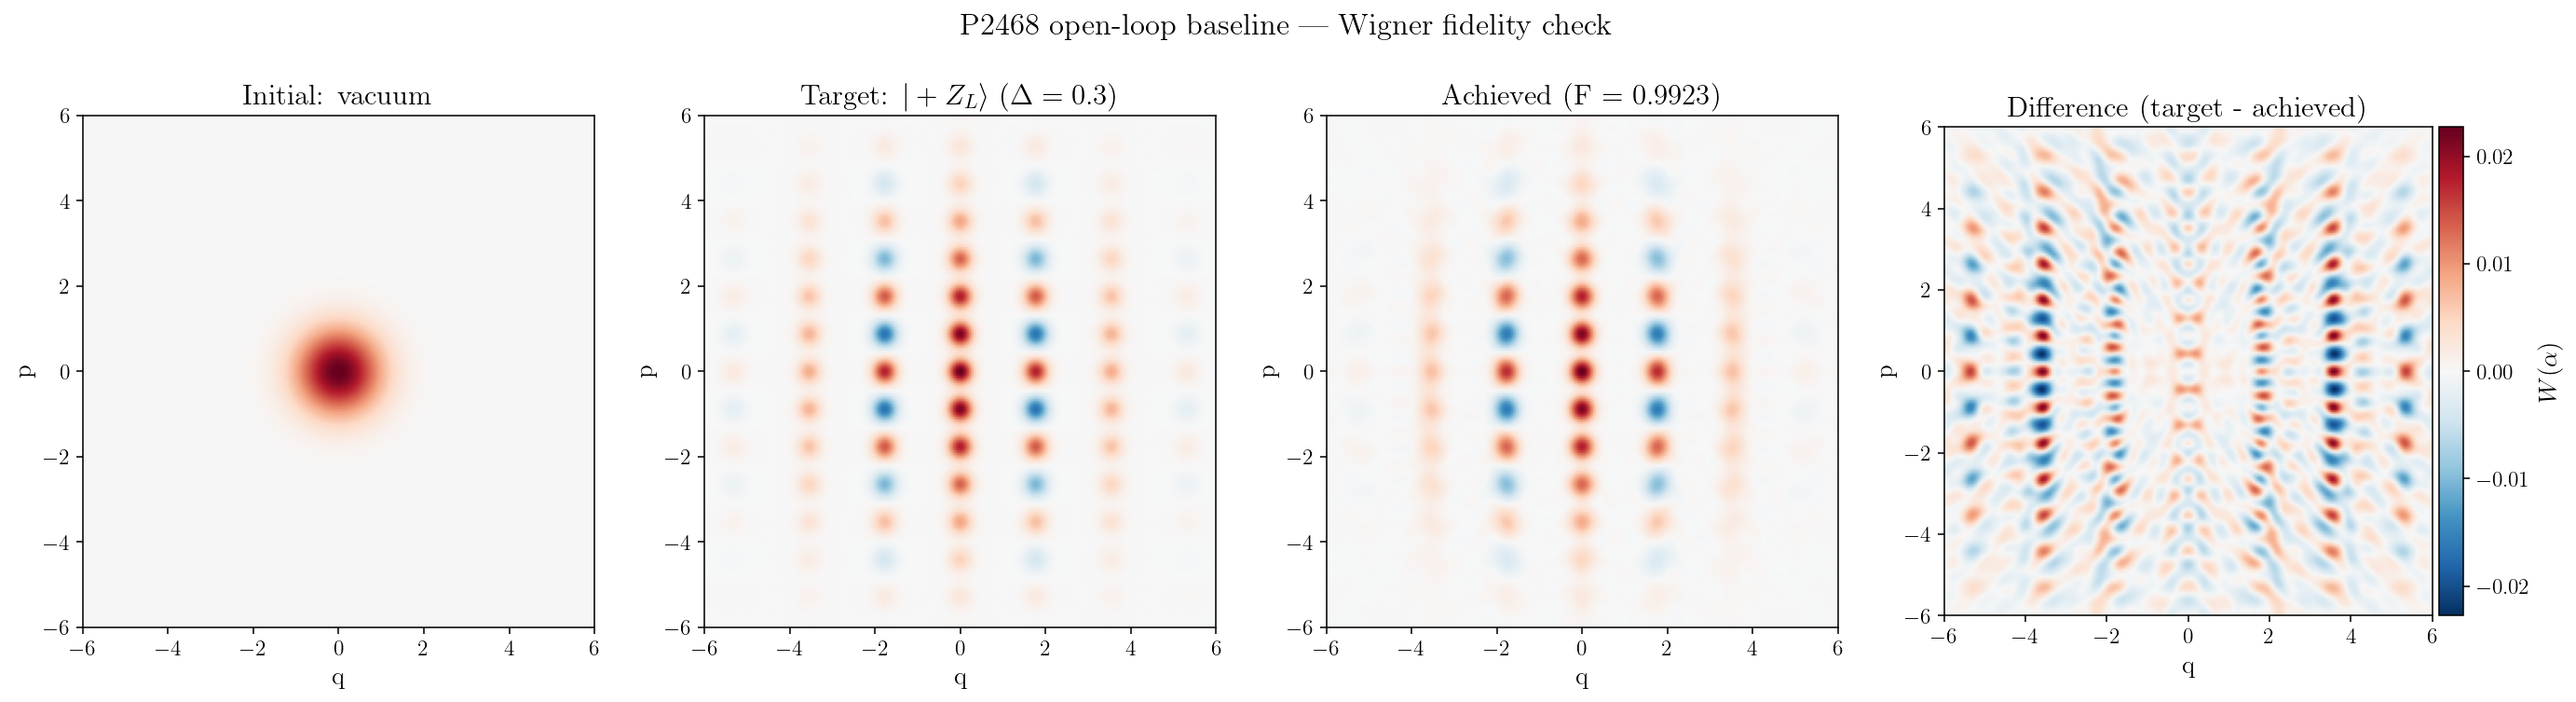
\includegraphics[width=\linewidth]{wigner_check.png}
\caption{Wigner functions for the continuous-pulse baseline. The achieved state is
visually indistinguishable from the target; the difference panel peaks at
$\pm0.02$ against grid features of $\pm0.3$, with the residual confined to the
outer, high-photon-number peaks.}
\label{fig:wigner}
\end{figure}

\subsection{Minimum time shortens the path without straightening it}

Sweeping the horizon at fixed target (Figure~\ref{fig:mintime}), $\Rlen$ changes
by $25\times$ across the sweep while $\Dpath$ changes by only $1.35\times$. Time
pressure compresses the route; it does not move it onto the geodesic.

\begin{figure}[t]
\centering
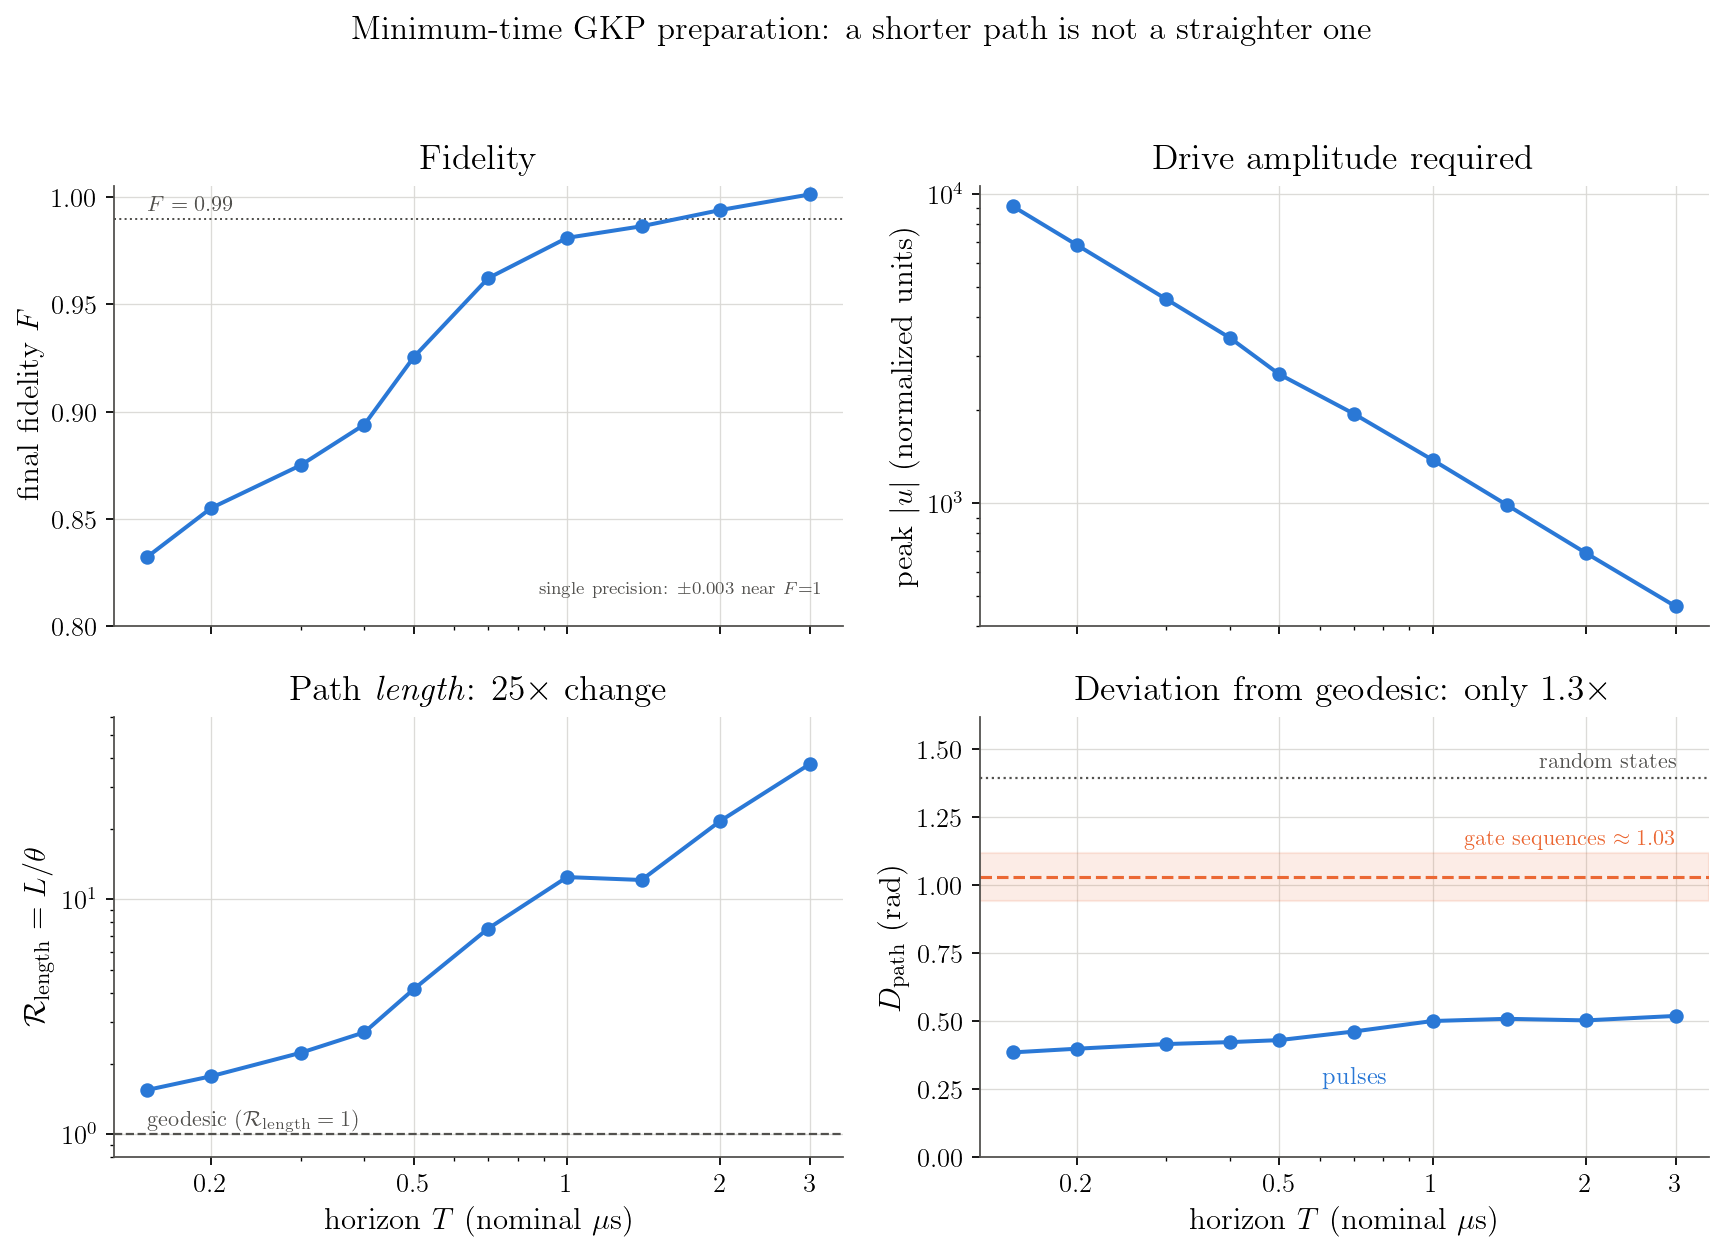
\includegraphics[width=\linewidth]{min_time_sweep.png}
\caption{Horizon sweep for the pump family. Path \emph{length} collapses by
$25\times$ as $T$ shrinks; deviation from the geodesic moves by $1.35\times$.
Efficiency is bought with amplitude.}
\label{fig:mintime}
\end{figure}

\subsection{Gate sequences are twice as far out, and nothing we varied moved them}

Table~\ref{tab:gates} summarizes $26$ gate configurations. $\Dpath$ is
$1.031\pm0.089$ throughout --- against $0.46$ for pulses and $1.395$ for random
states. On the scale from geodesic to random, gate trajectories are $74\%$ of the
way to random; pulses are $32\%$.

\begin{table}[t]
\centering
\small
\begin{tabular}{@{}llr@{}}
\toprule
Variation & Range covered & Effect on $\Dpath$ \\
\midrule
SNAP width (gate-set richness) & $2\to42$ phases ($21\times$) & $r=-0.09$ (none) \\
Gate algebra & displacement$+$SNAP vs.\ ECD & Welch $p=0.71$ (none) \\
Ancilla use & none vs.\ maximal entanglement ($\ln 2$) & $r=-0.12$ (none) \\
Circuit depth & $3\to16$ layers & weak \\
Fidelity & $0.56\to0.999$ & weak \\
\bottomrule
\end{tabular}
\caption{Invariance of $\Dpath$ across $26$ gate configurations
($1.031\pm0.089$). We predicted ECD would sit \emph{further} out, since
ancilla-mediated control routes through entangled states nearly orthogonal to the
product-state geodesic. ECD does reach maximal cavity entropy, and $\Dpath$ does
not move: entanglement is not the mechanism.}
\label{tab:gates}
\end{table}

\subsection{The structural obstruction, measured directly}

Staying on the geodesic requires matching its velocity. Projecting out the
unphysical component along $\ket{\psi}$, this is a linear least-squares problem in
the real amplitudes at every timestep,
\begin{equation}
\min_{u}\ \Big\| P\Big(H_{\mathrm{drift}}+\sum_k u_k O_k\Big)\ket{\psi}
 - P\,\HB\ket{\psi} \Big\|,
\qquad P = \mathbb{1}-\ket{\psi}\bra{\psi},
\label{eq:ls}
\end{equation}
solvable analytically --- no optimizer, no seeds, no local minima. The pump family
realizes only $62$--$79\%$ of the required velocity direction: $\HB$ is genuinely
not in the span of the control operators. The resulting tracker \emph{cannot
prepare the state}: fidelity peaks at $0.724$ and then degrades as it drifts and
overshoots. This is the most robust statement in this work, because it concerns
operator spans rather than what an optimizer happened to find.

\subsection{A claim of ours that did not survive}
\label{sec:pareto}

Every $\Dpath$ above was measured under a fidelity-only objective. We had
concluded that $\Dpath\approx0.45$ was the pump family's intrinsic distance from
time-optimality. Putting the geodesic \emph{into} the objective and sweeping the
weight,
\begin{equation}
\mathcal{L} = -F + \lambda\,\Dpath,
\end{equation}
refutes that (Table~\ref{tab:pareto}, Figure~\ref{fig:pareto}). The family reaches
$\Dpath=0.155$ at $F=0.992$: three times closer for eight tenths of a percent of
fidelity. The $0.459$ was slack, not structure. Note also that $\Rlen$
\emph{increases} as $\Dpath$ falls --- hugging the curve costs a longer path ---
which is direct evidence the two metrics are not proxies for one another.

This experiment places the geodesic in the objective by construction. It therefore
measures a \emph{reachability limit}, and must not be conflated with the
minimum-time results, which keep the geodesic in evaluation and support the
separate claim about what time pressure alone produces.

\begin{table}[t]
\centering
\small
\begin{tabular}{@{}rrrr@{}}
\toprule
$\lambda$ & $F$ & $\Dpath$ & $\Rlen$ \\
\midrule
$0$ (fidelity only) & $1.0000$ & $0.459$ & $56$ \\
$0.2$ & $0.9991$ & $0.295$ & $115$ \\
$0.5$ & $0.9980$ & $0.237$ & $161$ \\
$1.0$ & $0.9943$ & $0.192$ & $167$ \\
$2.0$ & $0.9920$ & $\mathbf{0.155}$ & $172$ \\
$5.0$ & $0.878$ & $0.075$ & $94$ \\
\bottomrule
\end{tabular}
\caption{Reachability frontier for the pump family. Path-optimality is nearly free
until $\Dpath\approx0.155$ and expensive thereafter. A row at $\lambda=10$ was
removed: it is dominated by the trivial solution below, and is therefore not a
Pareto point.}
\label{tab:pareto}
\end{table}

\begin{figure}[t]
\centering
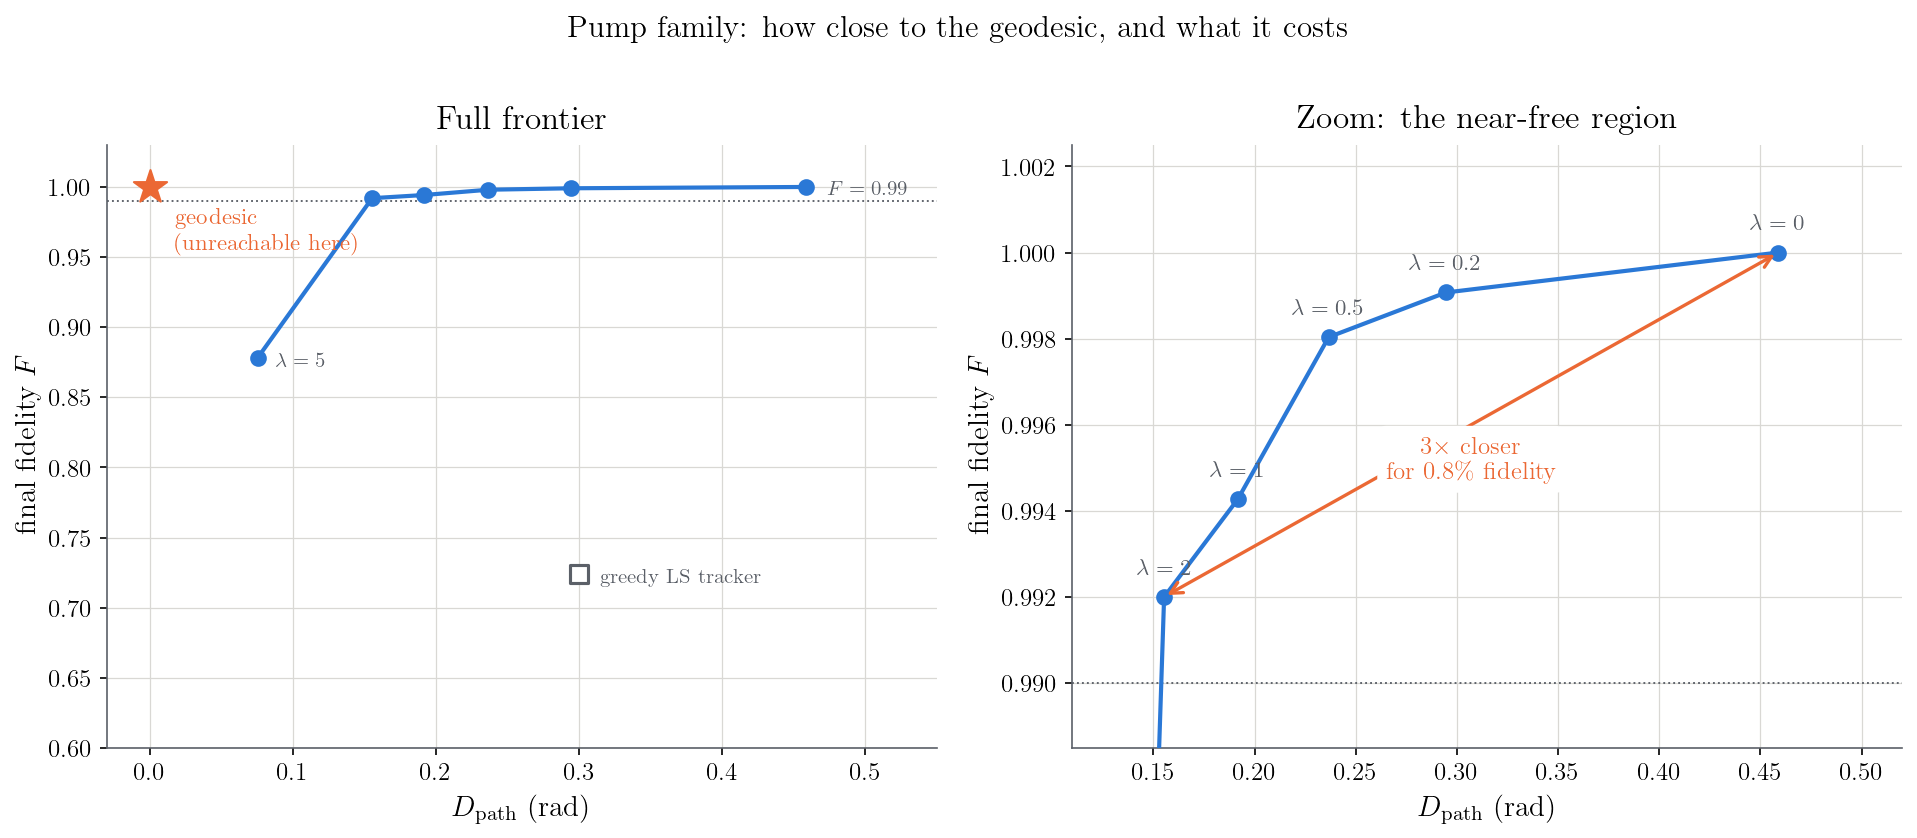
\includegraphics[width=\linewidth]{pareto.png}
\caption{Fidelity against geodesic deviation for the pump family. The greedy
least-squares tracker of Eq.~\eqref{eq:ls} is dominated by the globally optimized
frontier, confirming its single point was not the limit.}
\label{fig:pareto}
\end{figure}

\subsection{$\Dpath$ has a trivial minimizer}
\label{sec:trivial}

Any objective containing $\Dpath$ must contend with a degenerate solution: vacuum
\emph{is} $\ket{\gamma(0)}$, so a trajectory that does nothing at all scores
$\Dpath=0$ exactly, at $F=c_0^2=0.2962$. For $\lambda\gtrsim0.5$ this trivial
point beats any honest attempt on the raw objective, and a multi-start optimizer
falls straight into it --- as ours did, returning $F=0.2962$, $\Dpath=0$, $\Rlen=0$
for every large $\lambda$ in a first attempt. We therefore solve $\lambda=0$ first,
warm-start each subsequent $\lambda$ from the previous solution, and verify
explicitly that each reported point beats the trivial one. This is a general
hazard for path-deviation objectives, not a quirk of this system.

\subsection{Gates approach the geodesic, but not as closely}
\label{sec:gatepareto}

Applying the same sweep to a four-layer displacement$+$SNAP sequence
(Table~\ref{tab:gatepareto}) settles the comparison on equal footing: both
families optimized against a geodesic-aware objective, compared at matched
fidelity. Gates improve substantially on their fidelity-only value --- $1.116$ to
$0.693$ --- but the curve flattens as fidelity begins to erode, approaching an
asymptote near $0.7$. Pulses reach $0.155$ while still at $F=0.992$.

At $F\approx0.99$ the two families sit at $\Dpath\approx0.16$ and
$\Dpath\approx0.76$ respectively: a factor of four to five. Notably this gap is
\emph{wider} than the fidelity-only comparison suggested ($0.46$ versus $1.03$, a
factor of $2.2$). Testing both arms properly sharpened the distinction rather than
dissolving it, and it is the velocity-deficit of Eq.~\eqref{eq:ls} that supplies
the mechanism.

\begin{table}[t]
\centering
\small
\begin{tabular}{@{}rrrr@{}}
\toprule
$\lambda$ & $F$ & $\Dpath$ & $\Rlen$ \\
\midrule
$0$ (fidelity only) & $0.9964$ & $1.116$ & $20.1$ \\
$0.10$ & $0.9970$ & $0.906$ & $21.5$ \\
$0.20$ & $0.9947$ & $0.834$ & $19.3$ \\
$0.35$ & $0.9896$ & $0.788$ & $20.4$ \\
$0.50$ & $0.9866$ & $0.735$ & $19.8$ \\
$0.80$ & $0.9702$ & $\mathbf{0.693}$ & $15.9$ \\
\bottomrule
\end{tabular}
\caption{Reachability frontier for a four-layer displacement$+$SNAP sequence.
Every row beats the trivial solution of Section~\ref{sec:trivial}. Compare
Table~\ref{tab:pareto}: at matched fidelity $F\approx0.99$, pulses reach
$\Dpath\approx0.16$ where gates reach only $\approx0.76$.}
\label{tab:gatepareto}
\end{table}

\subsection{A learned policy does not close the gap}

For completeness we trained a PPO policy on a minimum-time formulation of the same
problem (destination-only reward: per-step $-\Delta t$, terminal bonus, and
potential-based shaping on the angle to the target). The environment was validated
by replaying the optimized pulse, which reproduces $F=0.9923$ exactly. From a
random start the policy reaches $F=0.593$ --- the squeezing ceiling again ---
because the default exploration scale is roughly $20\times$ the perturbation that
already destroys a good solution ($1\%$ amplitude noise costs $0.14$ fidelity,
$3\%$ costs $0.55$). Behaviour cloning from the optimized pulse reaches only
$0.32$ owing to covariate shift; noise-augmented cloning reaches $0.821$, and PPO
fine-tuning does not improve on it ($0.818$). Open-loop optimal control is already
optimal on this deterministic problem, so a tie was the best available outcome and
we did not achieve it.

\section{Physics diagnostics}

Numerical geometry should be checked against the physics it summarizes.
Figure~\ref{fig:gatepath} places the Wigner function after each gate beside the
geodesic sampled at equal arc length. Both rows begin at vacuum and end at the
target, so everything in between is the protocol's detour made visible: the
geodesic interpolates cleanly and symmetrically between the two, while the gate
sequence displaces the state far across phase space before reassembling the
lattice.

\begin{figure}[t]
\centering
\makebox[\linewidth][c]{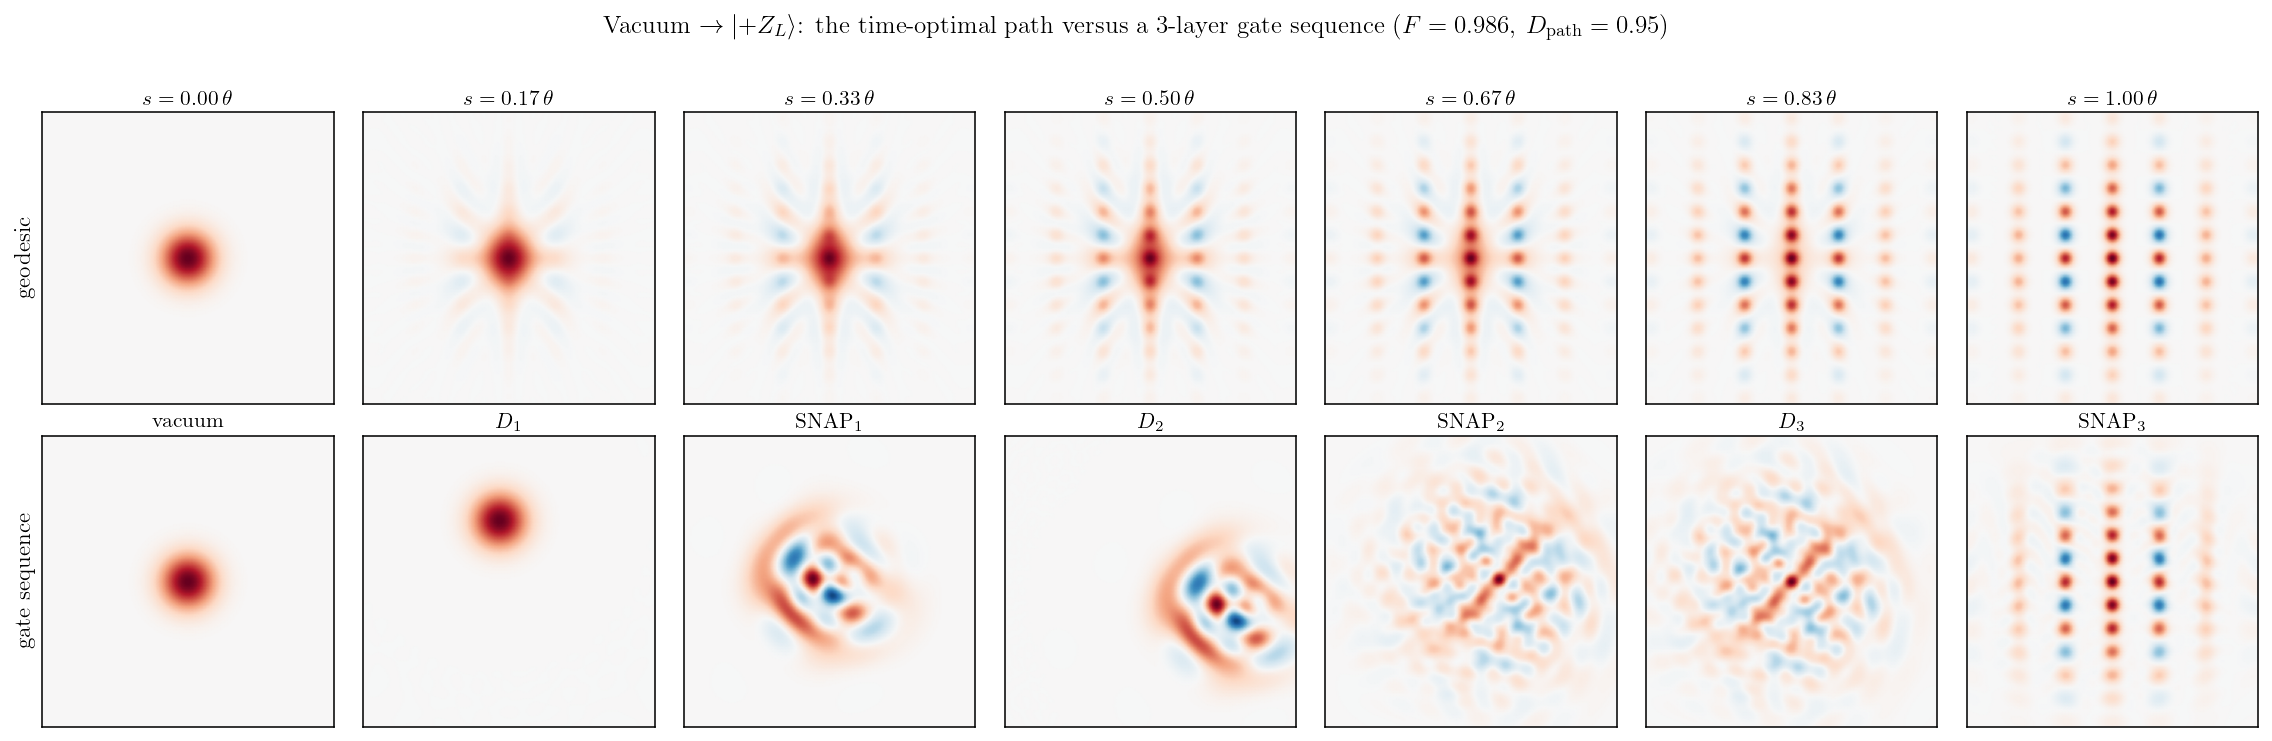
\includegraphics[width=1.28\linewidth]{gate_path_wigner.png}}
\caption{The time-optimal path (top) against a displacement$+$SNAP sequence
(bottom) reaching comparable fidelity. This is the qualitative content of
$\Dpath$.}
\label{fig:gatepath}
\end{figure}

\section{Planned work}

\paragraph{Geodesic waypoints as a fidelity objective.} The natural next
experiment keeps everything in the language of fidelity. Rather than penalizing
$\Dpath$, prescribe waypoints $s_1<\dots<s_m$ along the geodesic and optimize
\begin{equation}
\mathcal{L} = -\sum_{j=1}^{m} w_j \,\big|\braket{\gamma(s_j)|\psi(t_j)}\big|^2 ,
\label{eq:waypoints}
\end{equation}
so every term is an ordinary state-transfer fidelity. Two reasons to expect this
to help: it decomposes a long-horizon credit assignment problem into short stages,
much as the $\Delta$-curriculum did; and it is physically transparent, since each
target is a specific state whose Wigner function can be inspected. As with
Section~\ref{sec:pareto}, this places the geodesic in the objective and therefore
measures reachability.

\paragraph{ECD under the same test.} Section~\ref{sec:gatepareto} settles the
comparison for displacement$+$SNAP. Repeating it for ECD would establish whether
the $\approx0.7$ asymptote is a property of gate-based control generally or of
that one instruction set, and is the natural completion of Table~\ref{tab:gates}.

\paragraph{Wigner diagnostics along every protocol.} Extending
Figure~\ref{fig:gatepath} to ECD and to the waypoint-optimized sequences gives a
qualitative check on whether ``closer in $\Dpath$'' corresponds to
``visibly cleaner and more symmetric'' --- the physical claim the metric is meant
to formalize.

\section{Limitations}

Everything reported here concerns a single target, $\zL$ at $\Delta=0.3$ with
$n_{\mathrm{fock}}=100$. Absolute times are nominal: the operators are subspace
normalized, so only dimensionless ratios ($\Rlen$, $\Dpath$, $\mathcal{R}_T$) are
meaningful. $\mathcal{R}_T$ is additionally convention-sensitive, since the
realized energy uncertainty is far below the family's worst-case bound. All
fidelities are multi-start local optima, not certified global ones; the reinforcement
learning arm is a single seed at modest tuning effort. Two questions remain open
for methodological rather than physical reasons: whether the continuous/discrete
distinction survives a within-family test, and whether feedback helps under control
noise, whose open-loop comparator overfit its training perturbations. Finally, the
static baseline reported by the numerical layer was never reproduced exactly; the
protocol details are not recorded in the shared repository.

\end{document}
